\documentclass[12pt]{article}
\usepackage[paper=letterpaper,margin=2cm]{geometry}
\usepackage{amsmath}
\usepackage{amssymb}
\usepackage{amsfonts}
\usepackage{newtxtext, newtxmath}
\usepackage{enumitem}
\usepackage{titling}
\usepackage[colorlinks=true]{hyperref}
\usepackage[T1]{fontenc}
\usepackage{listings}
\usepackage{color}
\usepackage{graphicx}
\usepackage{tikz}
\usepackage{multicol}
\usepackage{colortbl}
\usepackage{booktabs}
\usepackage{array}
\usepackage{caption}
\usepackage{xcolor}

\hypersetup{
    colorlinks,
    linkcolor={red!90!black},
    citecolor={green!70!black},
    urlcolor={blue!80!black}
}

\definecolor{dkgreen}{rgb}{0,0.6,0}
\definecolor{gray}{rgb}{0.5,0.5,0.5}
\definecolor{mauve}{rgb}{0.58,0,0.82}

\lstset{frame=tb,
  language=Python,
  upquote=true,
  showstringspaces=false,
  columns=flexible,
  basicstyle={\small\ttfamily},
  numbers=left,
  numberstyle=\tiny\color{gray},
  keywordstyle=\color{blue},
  commentstyle=\color{dkgreen},
  stringstyle=\color{mauve},
  breaklines=true,
  breakatwhitespace=true,
  tabsize=2,
  backgroundcolor=\color{white},   % choose the background color
  captionpos=b,                    % sets the caption-position to bottom
  escapeinside={\%*}{*)},          % if you want to add LaTeX within your code
}


\title{CS421 Project - Anomalous User Prediction}
\author{Loh Jin Han, Goh Wei Han, Choo Wai Hong\\Wong Ginn Munn, Sean Seah Yuan Jin}
\date{16 November 2023}

\begin{document}
\maketitle
\tableofcontents
\pagebreak
\section{Problem Statement}
In this project, our goal was to detect anomalous users in recommender system datasets by classifying unseen data. Using labelled datasets containing user-item interactions and anomaly labels, we trained a machine learning model to identify anomalous users in an unlabelled dataset. Evaluation focused on ROC-AUC, while considering F1 score, precision, and recall values.

\section{Literature Review}
Our approach for this project was to attempt to apply the methods we are learnt in class, and supplement that with our research findings, to come up with the optimal model for the task. We first focused on finding more general research regarding anomaly detection, and came across one depicting it as a Machine Learning use case. \cite{kuangHaoAnomalyDetection} The article introduces us to the key things to look for when doing anomaly detection, such as doing Principal Component Analysis (PCA) to reduce dimensionality. By performing PCA, we can find the principal components that define the data and ignore the noise. The article proposes different Machine Learning algorithms such as K-nearest Neighbours (KNN), Support Vector Machine (SVM), Isolation Forest, and Recurrent Neural Networks (RNN), which we explored during our project. The article also mentioned different applications of anomaly detection, such as fraud detection and intrusion detection.

As we were given imbalanced datasets, we researched case studies involving imbalanced datasets. We came across a study regarding credit card frauds, and they used KNN, SVM, ANN, as well as multiple classifier systems to get better predictions. \cite{8985298} We also found three ways to handle the imbalanced data: resampling (undersampling and oversampling), cost-sensitive training, and tree algorithms (decision tree, random forest and Naive-Bayes). \cite{Mînăstireanu_Meşniţă_2020} Overall, we have researched many different algorithms and approaches we can use to tackle the anomaly detection task.
\section{Methodology}
\subsection{Data pre-processing}
We were given two dataframes, one containing the columns user, item, ratings, and another with the user and label. We first merge into one dataframe containing the columns user, item, rating, label, by merging on the column user. Table \ref{table:1} shows our merged labelled dataframe.
\subsection{Feature engineering}
The next step in our data pre-processing is to aggregate the training data. We create a column for each item in the dataset, and do a one-hot encoding of the user ratings for each item. A user can give a rating of $\{1, 0, -1\}$ if he likes, is neutral, or dislikes an item respectively. For items that a user didn't give a rating for, it was originally \lstinline{NaN} but we discovered that setting them to -1 gives the best results. An intuition on this is that users who choose not to watch a movie probably dislike it and would give a rating of -1.

Then, we added additional engineered features. We explored the \lstinline{scipy.stats} package to find out which summary statistics, when added, would increase the performance of our model. Code \ref{code:1} shows our complete feature engineering function. We then normalised the features using \lstinline{standard scalar}, as the summary statistics and the user-item ratings do not have a consistent scale.

However, we still had a matrix with over a thousand features. This impacted our model performance as well as the computational complexity for model training. Hence, we made use of PCA to perform dimensionality reduction and found that retaining the top 8 Principle Components was optimal (Figure \ref{figure:1}). We eventually tried Kernel PCA due to the large number of features. Despite being less computationally efficient, it allowed us to handle higher dimensional data and achieve a better AUC score in general. Ultimately, we found these optimal hyperparameters for Kernel PCA:
\begin{itemize}
  \item Number of principal components to retain was set at 34
  \item Dense eigensolver is used to run the exact full eigenvalue decomposition
  \item Radial Basis Function (RBF) for kernel to enable us to assign higher weights to data points that are close to a reference point
  \item Gamma $\gamma$ set to 0.0023. $\gamma$ is the coefficient of the RBF kernel and it determines the shape of the kernel function
\end{itemize}
Using the optimal hyperparameters, we obtain our final design matrix (Table \ref{table:2}) used for model training.

\subsection{Machine Learning Methods}
We explored a plethora of machine learning models for this project, which includes at least two supervised (ANN, SVM, etc.) and two unsupervised learning methods (K-Means Clustering, DBSCAN, etc.). Eventually, we settled to focus on three models, ANN, Isolation Forest, and SVM that we believe best suits the requirements for this problem.

\subsection{Model training methodology}
Before any model training, we performed a train-test-validation split of $60, 20, 20$. This ensures that we can have an unbiased estimate of model performance on the test set, and only train and tune the hyperparameters on the training and validation set respectively. We were very careful in our code not to leak any data and made sure the test set was untouched.

\subsubsection{Artificial Neural Networks}
We tried this first because we had prior experience building neural networks (Code \ref{code:2}).The difficulty in training this model is the number of hyperparameters to tune. We had to decide how many layers, how many nodes on each layer, what activation function, drop out layers and regularisation for each layer. In the later weeks, our best AUC was 0.88.

\subsubsection{Isolation Forest}
Isolation Forest is ideal for identifying anomalous users in recommender systems due to its efficiency with high-dimensional data, sensitivity to anomalies, and scalability. Its unsupervised nature suits scenarios with rare anomalies, and its interpretability aligns with the evaluation metrics. Its simplicity allows for easy implementation and exploration of other ensemble methods, such as Random Forests, to enhance classification performance. Our best AUC was also 0.88.

\subsubsection{Support Vector Machine}
SVM is a supervised learning machine algorithm that works by finding a hyperplane in a high-dimensional space that best separates data points into different classes. We used a special implementation called Support Vector Classification (SVC) for this classification task. Given a set of training data with features $x_i$ and labels $y_i \in \{-1, 1\}$, we find a hyperplane represented by the equation where $w$ is the weight vector and $b$ is the bias
$$
  w\cdot x + b = 0
$$
The main objective in optimising this equation is to find the most optimal $w$ and $b$ to maximise the margin while correctly classifying the training data. The cost function to minimise will be
$$
  \text{Minimise}: \frac{1}{2}\lVert w\rVert^2
$$
We have to fine tune a few hyperparameters for the optimisation problem. We compared validation scores against train scores amongst the hyperparameters with AUC comparison.

\begin{itemize}
  \item $C$: $C$ is the regularisation parameter that regulates the trade-off between maximising the margin and minimising error. It influences the balance between $\lVert w\rVert^2$ and correctly classifying the training points. We found $C=1.5$ to be optimal (Figure \ref{figure:2}).
  \item Gamma $\gamma$: $\gamma$ in SVM's RBF kernel shapes the decision boundary by determining the reach of individual training points. It acts as the exponent in the RBF kernel, influencing $w\cdot x$ through the Euclidean distance term. We found $\gamma = 21.96$ to be optimal (Figure \ref{figure:3}).
\end{itemize}
With Kernel PCA, we achieved our highest AUC score of $0.95$ in week 12.

\subsection{Testing Methodology}
After we trained and tuned our model, we used it to predict the labels on our test dataset. The processing of the test set was the same as that of the training and validation sets, incorporating the aggregation, feature engineering and PCA. The data was also sorted by userId in ascending order. Subsequently, the test set underwent evaluation using the trained models. For the SVM Model that produced the best AUC score, its values were adjusted based on the optimal threshold determined during training. These adjusted values were then fed into a helper method \lstinline{generate_test_output()}, which generates the CSV file intended for submission.

\section{Conclusion}
In conclusion, our team learnt the importance of taking a step-by-step approach to construct a successful machine learning model. Through adept feature engineering, data cleaning and transformations of the datasets given, it enabled us to improve the accuracy and stability of our final model. As the dataset was imbalanced, these steps were crucial to building a good model as it allowed us to address problems such as bias and overfitting. By exploring different models and evaluating its pros and cons, we were able to find the best suited model and eventually settled for SVM. Finally, with our best model, we focused on hyperparameter tuning for maximum AUC. Overall, our approach collectively contributed to the development of a successful machine learning model.
\pagebreak
\section{Appendix}
\begin{table}[ht!]
  \centering
  \bgroup
  \def\arraystretch{1.5}%
  \begin{tabular}{|c|c c c|}
    \hline
    {user} & item & rating & label \\
    \hline
    1220   & 6    & 0      & 0     \\
    1220   & 21   & 1      & 0     \\
    ...    & ...  & ...    & ...   \\
    5071   & 141  & -1     & 1     \\
    5071   & 158  & -1     & 1     \\
    \hline
  \end{tabular}
  \egroup
  \caption{Merged Labelled dataset}
  \label{table:1}
\end{table}

\label{code:1}\begin{lstlisting}[caption={Feature Engineering function}]
def agg_rating_stats(X, y):
    unique_items = X.item.unique() #unique movies
    columns = np.append(unique_items, 'label')
    result = pd.DataFrame(columns=columns)
    lst = []
    total = len(X.item.unique())

    for user in X.user.unique():
        ratings = X[X['user'] == user]['rating'] # ratings by single user
        ratings_df = X[X['user'] == user] # user -> item -> rating df for single user
        ratings_df.loc[:, 'item'] = ratings_df['item'].astype(str) # convert movie id from number to string
        ratings_dict = dict(zip(ratings_df.item, ratings_df.rating))
        label = y[y['user'] == user].iloc[0]['label']
        ratings_dict['label'] = label
        ratings_dict['user'] = user
        ratings_dict['rating_count'] = len(ratings)
        ratings_dict['rating_proportion_of_total'] = len(ratings) / total
        ratings_dict['rating_mean'] = np.mean(ratings)
        ratings_dict['rating_sem'] = sem(ratings)
        ratings_dict['rating_sd'] = np.std(ratings)
        ratings_dict['rating_variance'] = np.var(ratings)
        ratings_dict['rating_sum'] = sum(ratings)
        ratings_dict['negative_count'] = sum(rating < 0 for rating in ratings)
        ratings_dict['negative_proportion'] = sum(rating < 0 for rating in ratings) / len(ratings)
        ratings_dict['negative_proportion_of_total'] = sum(rating < 0 for rating in ratings) / total
        ratings_dict['neutral_count'] = sum(rating == 0 for rating in ratings)
        ratings_dict['neutral_proportion'] = sum(rating == 0 for rating in ratings) / len(ratings)
        ratings_dict['neutral_proportion_of_total'] = sum(rating == 0 for rating in ratings) / total
        ratings_dict['positive_count'] = sum(rating > 0 for rating in ratings)
        ratings_dict['positive_proportion'] = sum(rating > 0 for rating in ratings) / len(ratings)
        ratings_dict['positive_proportion_of_total'] = sum(rating > 0 for rating in ratings) / total
        ratings_dict['skew'] = skew(ratings)
        ratings_dict['entropy'] = entropy([ratings_dict['negative_proportion_of_total'], ratings_dict['positive_proportion_of_total'], 1-ratings_dict['negative_proportion_of_total']- ratings_dict['positive_proportion_of_total']])
        ratings_dict['kurtosis'] = kurtosis(ratings)
        ratings_dict['iqr'] = iqr(ratings)
        lst.append(ratings_dict)

    result = pd.concat([result, pd.DataFrame(lst)], ignore_index=True)
    result = result.fillna(-1)
    return result
\end{lstlisting}

\begin{figure}[ht!]
  \begin{center}
    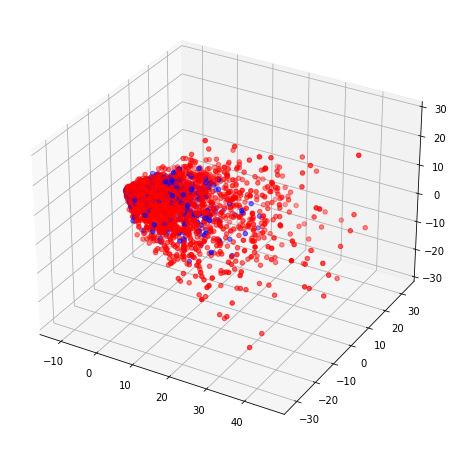
\includegraphics[scale=0.7]{"./Diagrams/PCA.png"}
    \caption{PCA Analysis}
    \label{figure:1}
  \end{center}
\end{figure}
\pagebreak

\begin{table}[ht!]
  \centering
  \bgroup
  \def\arraystretch{1.5}%
  \begin{tabular}{|c|c c c c c|}
    \hline
         & 0          & 1          & ... & 40        & 41        \\
    \hline
    0    & 16.118170  & -16.739490 & ... & -1.179041 & 4.235142  \\
    1    & -4.308369  & -5.760263  & ... & -0.809216 & 0.402063  \\
    ...  & ...        & ...        & ... & ...       & ...       \\
    3058 & -4.783880  & -3.383966  & ... & 0.735087  & -0.023320 \\
    3059 & -10.318746 & -0.831301  & ... & -0.377284 & -0.961972 \\
    \hline
  \end{tabular}
  \egroup
  \caption{Final design matrix showing principal components}
  \label{table:2}
\end{table}


\label{code:2}\begin{lstlisting}[caption={Neural Network Structure}]
# Final Neural Network structure
model = tf.keras.models.Sequential()

model.add(tf.keras.layers.Dense(128, input_dim=X_train_PC.shape[1], activation='tanh', kernel_regularizer=tf.keras.regularizers.l1(0.002)))
model.add(tf.keras.layers.Dense(128, activation='tanh', kernel_regularizer=tf.keras.regularizers.l1(0.001)))
model.add(tf.keras.layers.Dense(128, activation='tanh', kernel_regularizer=tf.keras.regularizers.l1(0.001)))
model.add(tf.keras.layers.Dense(1, activation='sigmoid'))

model.summary()
#AUC 0.88
\end{lstlisting}

\begin{figure}[ht!]
  \begin{center}
    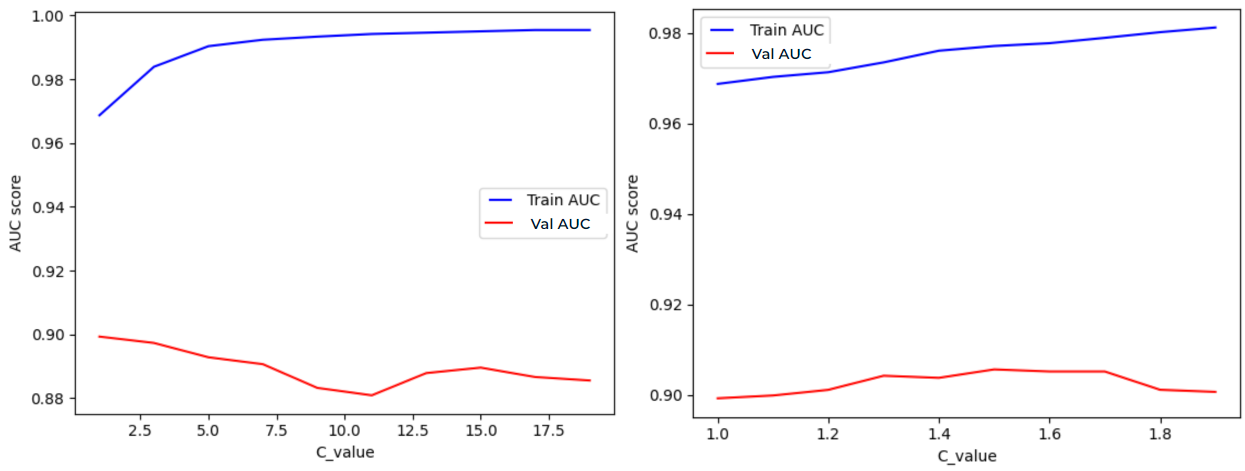
\includegraphics[scale=0.5]{"./Diagrams/c_graph.PNG"}
    \caption{SVM $C$ parameter}
    \label{figure:2}
  \end{center}
\end{figure}

\begin{figure}[ht!]
  \begin{center}
    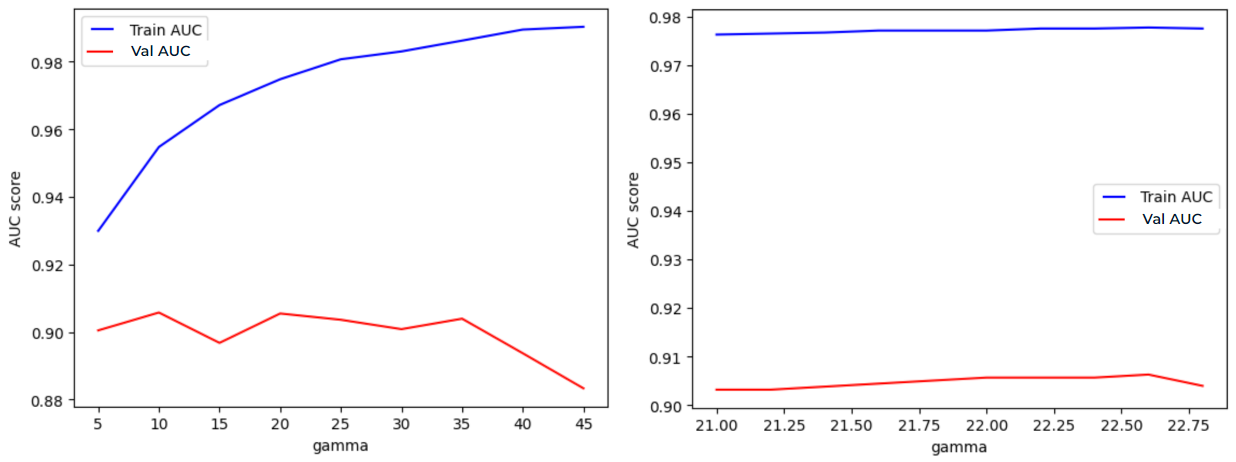
\includegraphics[scale=0.5]{"./Diagrams/gamma_graph.PNG"}
    \caption{SVM $\gamma$ parameter}
    \label{figure:3}
  \end{center}
\end{figure}

\pagebreak

\bibliographystyle{apalike}
\bibliography{refs}
\end{document}
